% -- Document configuration
\documentclass{article}

% -- Input and language settings
% \usepackage[utf8]{inputenc}
\usepackage[spanish]{babel}
\decimalpoint                             % From babel package to use points instead of commas in decimals

% -- Page and line settings
\usepackage{geometry}
\geometry{letterpaper, 
    % margin=2cm, 
    left=3cm, right=3cm,
    top=1.2cm, bottom=1.2cm,
    includefoot, 
    includehead}
\renewcommand{\baselinestretch}{1.2}

% -- Required packages
\usepackage{xcolor}
\usepackage[many]{tcolorbox}
\usepackage{mathtools,amsfonts,amsmath}     % Loads amsmath if not already loaded
\allowdisplaybreaks                         % To allow page breaks if equations are too long
\usepackage[parfill]{parskip}               % No indent and separation lines for paragraphs
\usepackage{cancel}                         % To cancel math terms
\usepackage[shortlabels]{enumitem}          % To handle enumerations
\usepackage{tikz}
\usetikzlibrary{automata, arrows.meta, positioning}
\usepackage[mode=buildnew]{standalone}      % To import figures in standalone files
\usepackage[hidelinks]{hyperref}
\usepackage[spanish]{cleveref}              % To use autocompleted reference labels, language must be change as in babel package
\usepackage{caption}                        % Caption and subcaption to allow subfigures
\usepackage{subcaption}
\usepackage{float}                          % To specify the location of figures
\usepackage{multicol}                       % To use multicolumns
\usepackage[bottom]{footmisc}               % To locate footnotes at the bottom

% -- Title and heading settings
\usepackage{titling}
\usepackage{fancyhdr}
\pagestyle{fancy}

% -- Code and code formatting
\usepackage{minted}                         % To insert code
\usemintedstyle[julia]{gruvbox-light}       % Code theme and language
\definecolor{bg}{rgb}{0.98, 0.97, 0.88}     % Code block background

\usepackage{fontspec}                       % To allow the use of monospace fonts
\setmonofont{JuliaMono}[Path=./codefonts/, Extension=.ttf, UprightFont=*-Regular, ItalicFont=*-RegularItalic, Scale=0.75]

\usepackage{fancyvrb}                       % To change line number font
\renewcommand{\theFancyVerbLine}{\textcolor{gray}{\footnotesize\texttt{\arabic{FancyVerbLine}}}}

\definecolor{light-gray}{gray}{0.95}        % Color, box and style to show small code thingys inside normal text
\newcommand{\code}[1]{\colorbox{light-gray}{\texttt{#1}}}

% -- Bilbiography preferences
\usepackage[square,numbers]{natbib}
\bibliographystyle{unsrt}

% -- Footnotes without numbering
\newcommand\nnfootnote[1]{%
  \begin{NoHyper}
  \renewcommand\thefootnote{}\footnote{#1}%
  \addtocounter{footnote}{-1}%
  \end{NoHyper}
}

% -- Theorems
\newtheorem{theorem}{Theorem}

\lhead{\theinstitution\ -- \thedepartment}
\chead{}
\rhead{Programación para la IA\ -- \thetitle}
\lfoot{}
\cfoot{\thepage}
\rfoot{}

% -- Problem solution
\newenvironment{solution}
{\begin{quote}
\textbf{Solución:}\medskip

}
{

\hfill\rule{0.5\textwidth}{0.5pt}
\end{quote}}

% -- Equation result
\newcommand{\result}[1]
{
\tcbhighmath[colframe=white, colback=gray!15, sharp corners]
{#1}
}

% -- Function definitions
\newcommand{\dprod}[2]{{#1} \cdot {#2}}
\newcommand{\txtgray}[1]{\textcolor{gray}{#1}}

% -- Author information
\title{Actividad 5}
\author{Leonardo Flores Torres}
\newcommand\theinstitution{Universidad Veracruzana}
\newcommand\thedepartment{Inteligencia Artificial}
\newcommand\thecourse{Programación para la Inteligencia Artificial}

% -- Paths
% \newcommand\codelists{../programs/lists.rkt}

% Remove red color boxes of "syntax errors" in minted
\AtBeginEnvironment{minted}{%
  \renewcommand{\fcolorbox}[4][]{#4}}

% -- Document
\begin{document}

\thispagestyle{empty}

%Title
\begin{center}
\textsc{\theinstitution}\\[2mm]

\thedepartment

\rule{0.6\textwidth}{0.5pt}\\[2mm]

\thecourse \\[4mm]

{\Large \textbf{\thetitle}}\\[2mm]

\theauthor \\[2mm]

{\small \today}
\end{center}
\medskip

% -- 
\vspace{1cm}

\begin{enumerate}
    \item Cálculo de $\pi$ usando el \textit{método de Monte Carlo}.
    \begin{itemize}
        \item Generar los puntos aleatorios usando \textit{convergencia lineal}.
        \item Generar los puntos aleatorios usando \textit{secuencia de Halton}.
        \item Generar los puntos aleatorios usando el generador valores aleatorios de su lenguaje de programación de preferencia.
    \end{itemize}

    \item Para cada caso graficar las curvas de convergencia, hacer al menos $10^6$ iteraciones.
    \item Analizar y determinar qué método fue más preciso.
    \item Pensar cómo aproximar $\pi$ con un número de cifras significativas dadas, por ejemplo, con un número de 4 cifras significativas el valor correspondiente sería $3.14159$.
    \begin{solution}
        El área de un círculo está dada por
        \begin{equation*}
            A_{\circlefig} = \pi r^2 .
        \end{equation*}
        Mientras que el área de una cuadrado es
        \begin{equation*}
            A_{\squarefig} = l^2 .
        \end{equation*}
        Es necesario que el círculo se encuentre inscrito en el cuadrado, y que el diámetro del círculo sea igual al lado del cuadrado $d = l$, de aquí que $r = l/2$. Aunque no se requiere todo el círculo, se puede tomar un cuadrante que contenga un cuarto del círculo, y un cuarto del cuadrado como se muestra en la \cref{fig:relacion_cuadrado_circulo}.

        \begin{figure}[ht!]
            \centering
            \begin{tikzpicture}
                \draw[step=2, gray!80, thick] (0,0) grid (4,4);
                \draw[gray!80, thick] (2,2) circle (2);
                \draw[to-to] (4.5, 2) -- node[right] {$l/2$} (4.5, 4);
                \draw[to-to] (2,1.5) -- node[below] {$r$} (4, 1.5);
                \draw[black, very thick] (2,2) rectangle (4,4);
            \end{tikzpicture}
            \caption{Círculo inscrito en un cuadrado.}
            \label{fig:relacion_cuadrado_circulo}
        \end{figure}

        Ahora se toma la razón entre ambas áreas,
        \begin{align*}
            \frac{A_{\circlefig/4}}{A_{\squarefig/4}} & = \frac{\pi r^2}{4} \cdot \frac{1}{r^2} , \\
            & = \frac{\pi}{4} .
        \end{align*}
        El lector podrá comprobar que se llega a la misma expresión analítica si se toma la razón entre el cuadrado y el círculo completos. Si se lanzaran puntos de manera aleatoria al cuarto del cuadrado marcado en negro, algunos de ellos caerían dentro el cuarto del círculo mientras que otros quedarían fuera. Por lo que las áreas $A_{\squarefig/4}$ y $A_{\circlefig/4}$ pueden reinterpretarse como la cantidad de puntos contenidos por el cuarto del cuadrado y por el cuarto de círculo, respectivamente.

        Para aproximar $\pi$ con el \textit{método de Monte Carlo} se implementaron dos generadores de números pseudo aleatorios. El primero corresponde al \textit{generador lineal congruencial}, su implementación está basada en el trabajo hecho por Schlegel en su blog \cite{schlegel2008lcg} la cual a su vez está basada en una implementación dentro del estándar del lenguaje de programación \code{C} \cite{saucier2000computer}, siendo esta última referencia de la que se obtienen los parámetros adecuados para este generador. Por otro lado, el pseudo código para la implementación de la \textit{secuencia de Halton} fue visto en una pregunta del sitio StackOverflow \cite{stack2013halton} y de Wikipedia \cite{wiki2013halton}.

        Para calcular los puntos aleatorios se añadieron 3 funciones \code{rngJulia}, \code{rngLcg} y \code{rngHalton}, como se muestra en el codigo adjunto en el apéndice. Posteriormente se juntaron en una sola función que llamaría a la necesaria dependiendo se un \code{keyword argument} como se muestra a continuación:
        \begin{minted}[
            frame=none,
            autogobble,
            obeytabs=false,
            breaklines,
            tabsize=4,
            linenos=true,
            baselinestretch=1,
            firstnumber=1,
            bgcolor=bg!70,
            ]{julia}
            julia> begin
                   n = 3_500_000    # numero de puntos deseados
                   
                   data_jul = ap.piesApprox(n; rng="julia")     # generador aleatorio de julia
                   data_lcg = ap.piesApprox(n; rng="lcg")       # generador aleatorio lcg
                   data_halt = ap.piesApprox(n; rng="halton")   # generador aleatorio de halton
                   
                   # Errores asociados a cada generador
                   err_jul = map(x -> abs(x - π), data_jul.pies)
                   err_lcg = map(x -> abs(x - π), data_lcg.pies)
                   err_halt = map(x -> abs(x - π), data_halt.pies)
                   end;
        \end{minted}

        Las aproximaciones de $\pi$ se muestran la \cref{fig:pi_approximations}, y sus respectivos errores en la \cref{fig:pi_errors}. Lo que se pudo observar es que el valor de todas las aproximaciones dependen de las semillas dadas en cada método. Por ejemplo, el método de la convergencia lineal tiene como semilla el tiempo del ordenador en milisegundos, el método de la secuencia de Halton tiene como semilla la base. Por otro lado, desconozco como es que el generador de números aleatorios de \code{julia} es implementado, pero usa un método llamdado \textit{Mersenne Twister} \cite{wiki2013mersenne}.


        \clearpage
        \begin{figure}
            \centering
            \begin{subfigure}{0.45\textwidth}
                \centering
                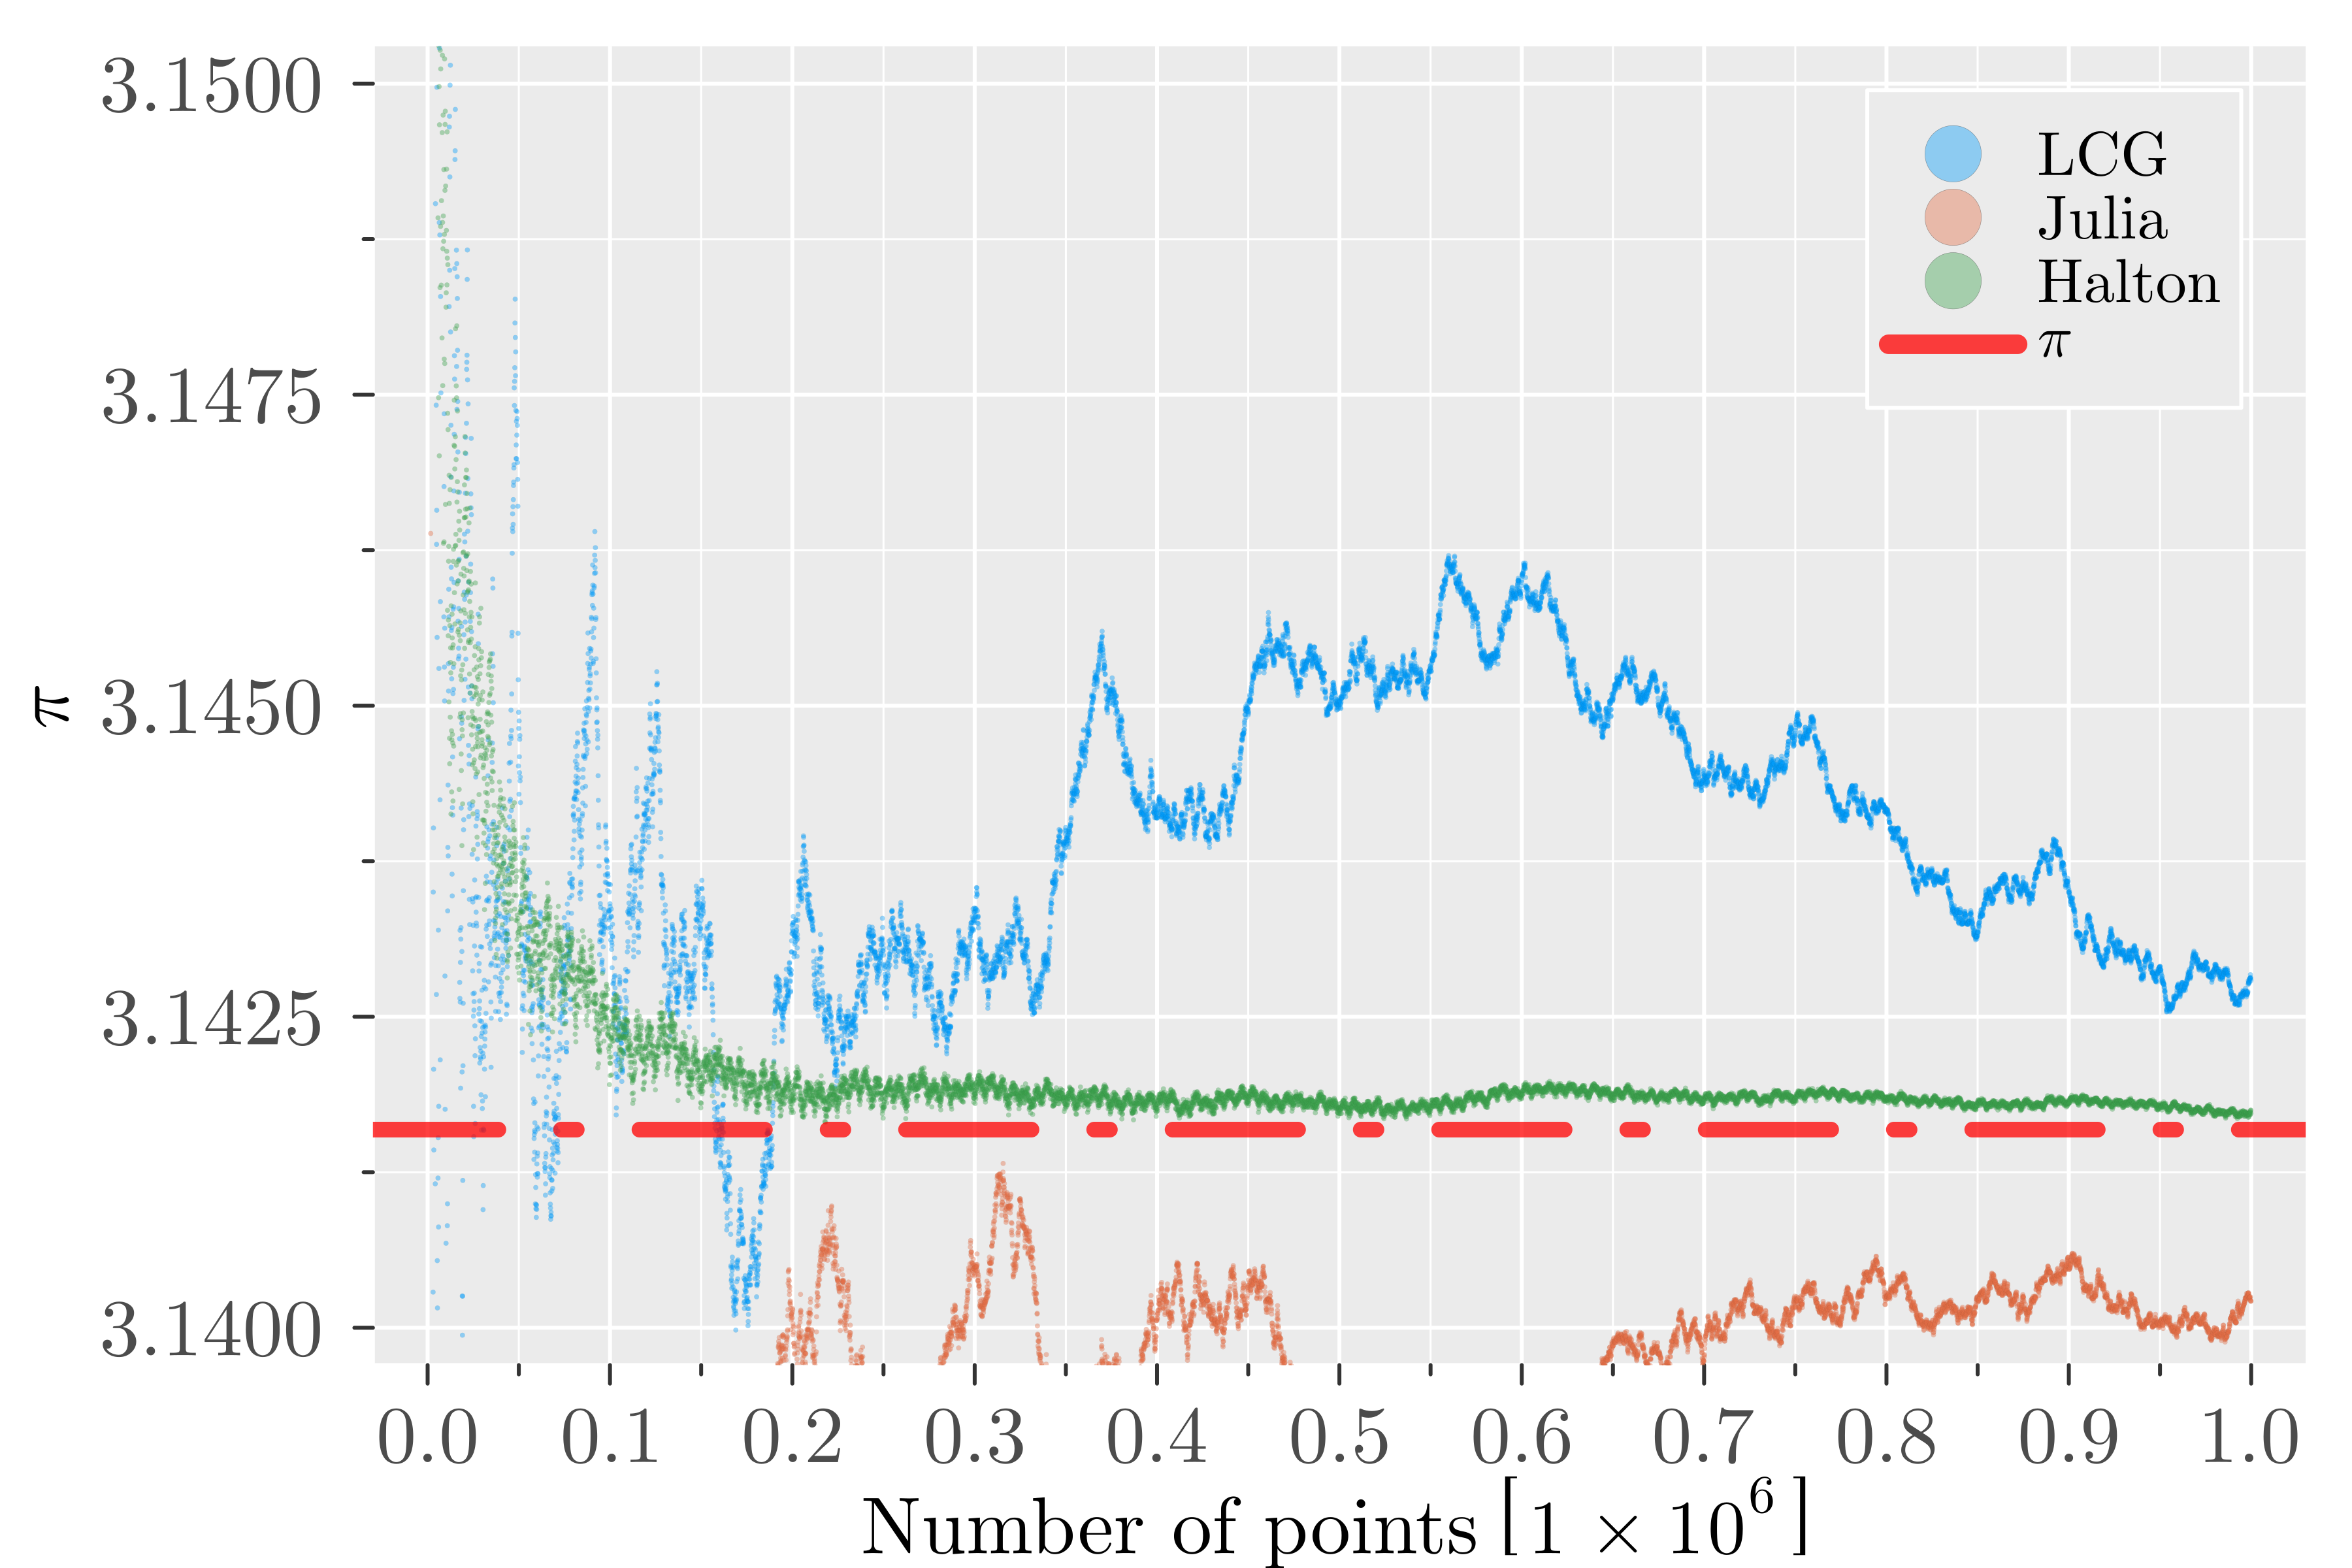
\includegraphics[scale=0.065]{../figures/pies_1E6.png}
                \caption{Aproximación de $\pi$ con $1 \times 10^6$ puntos.}
            \end{subfigure}
            \hfill
            \begin{subfigure}{0.45\textwidth}
                \centering
                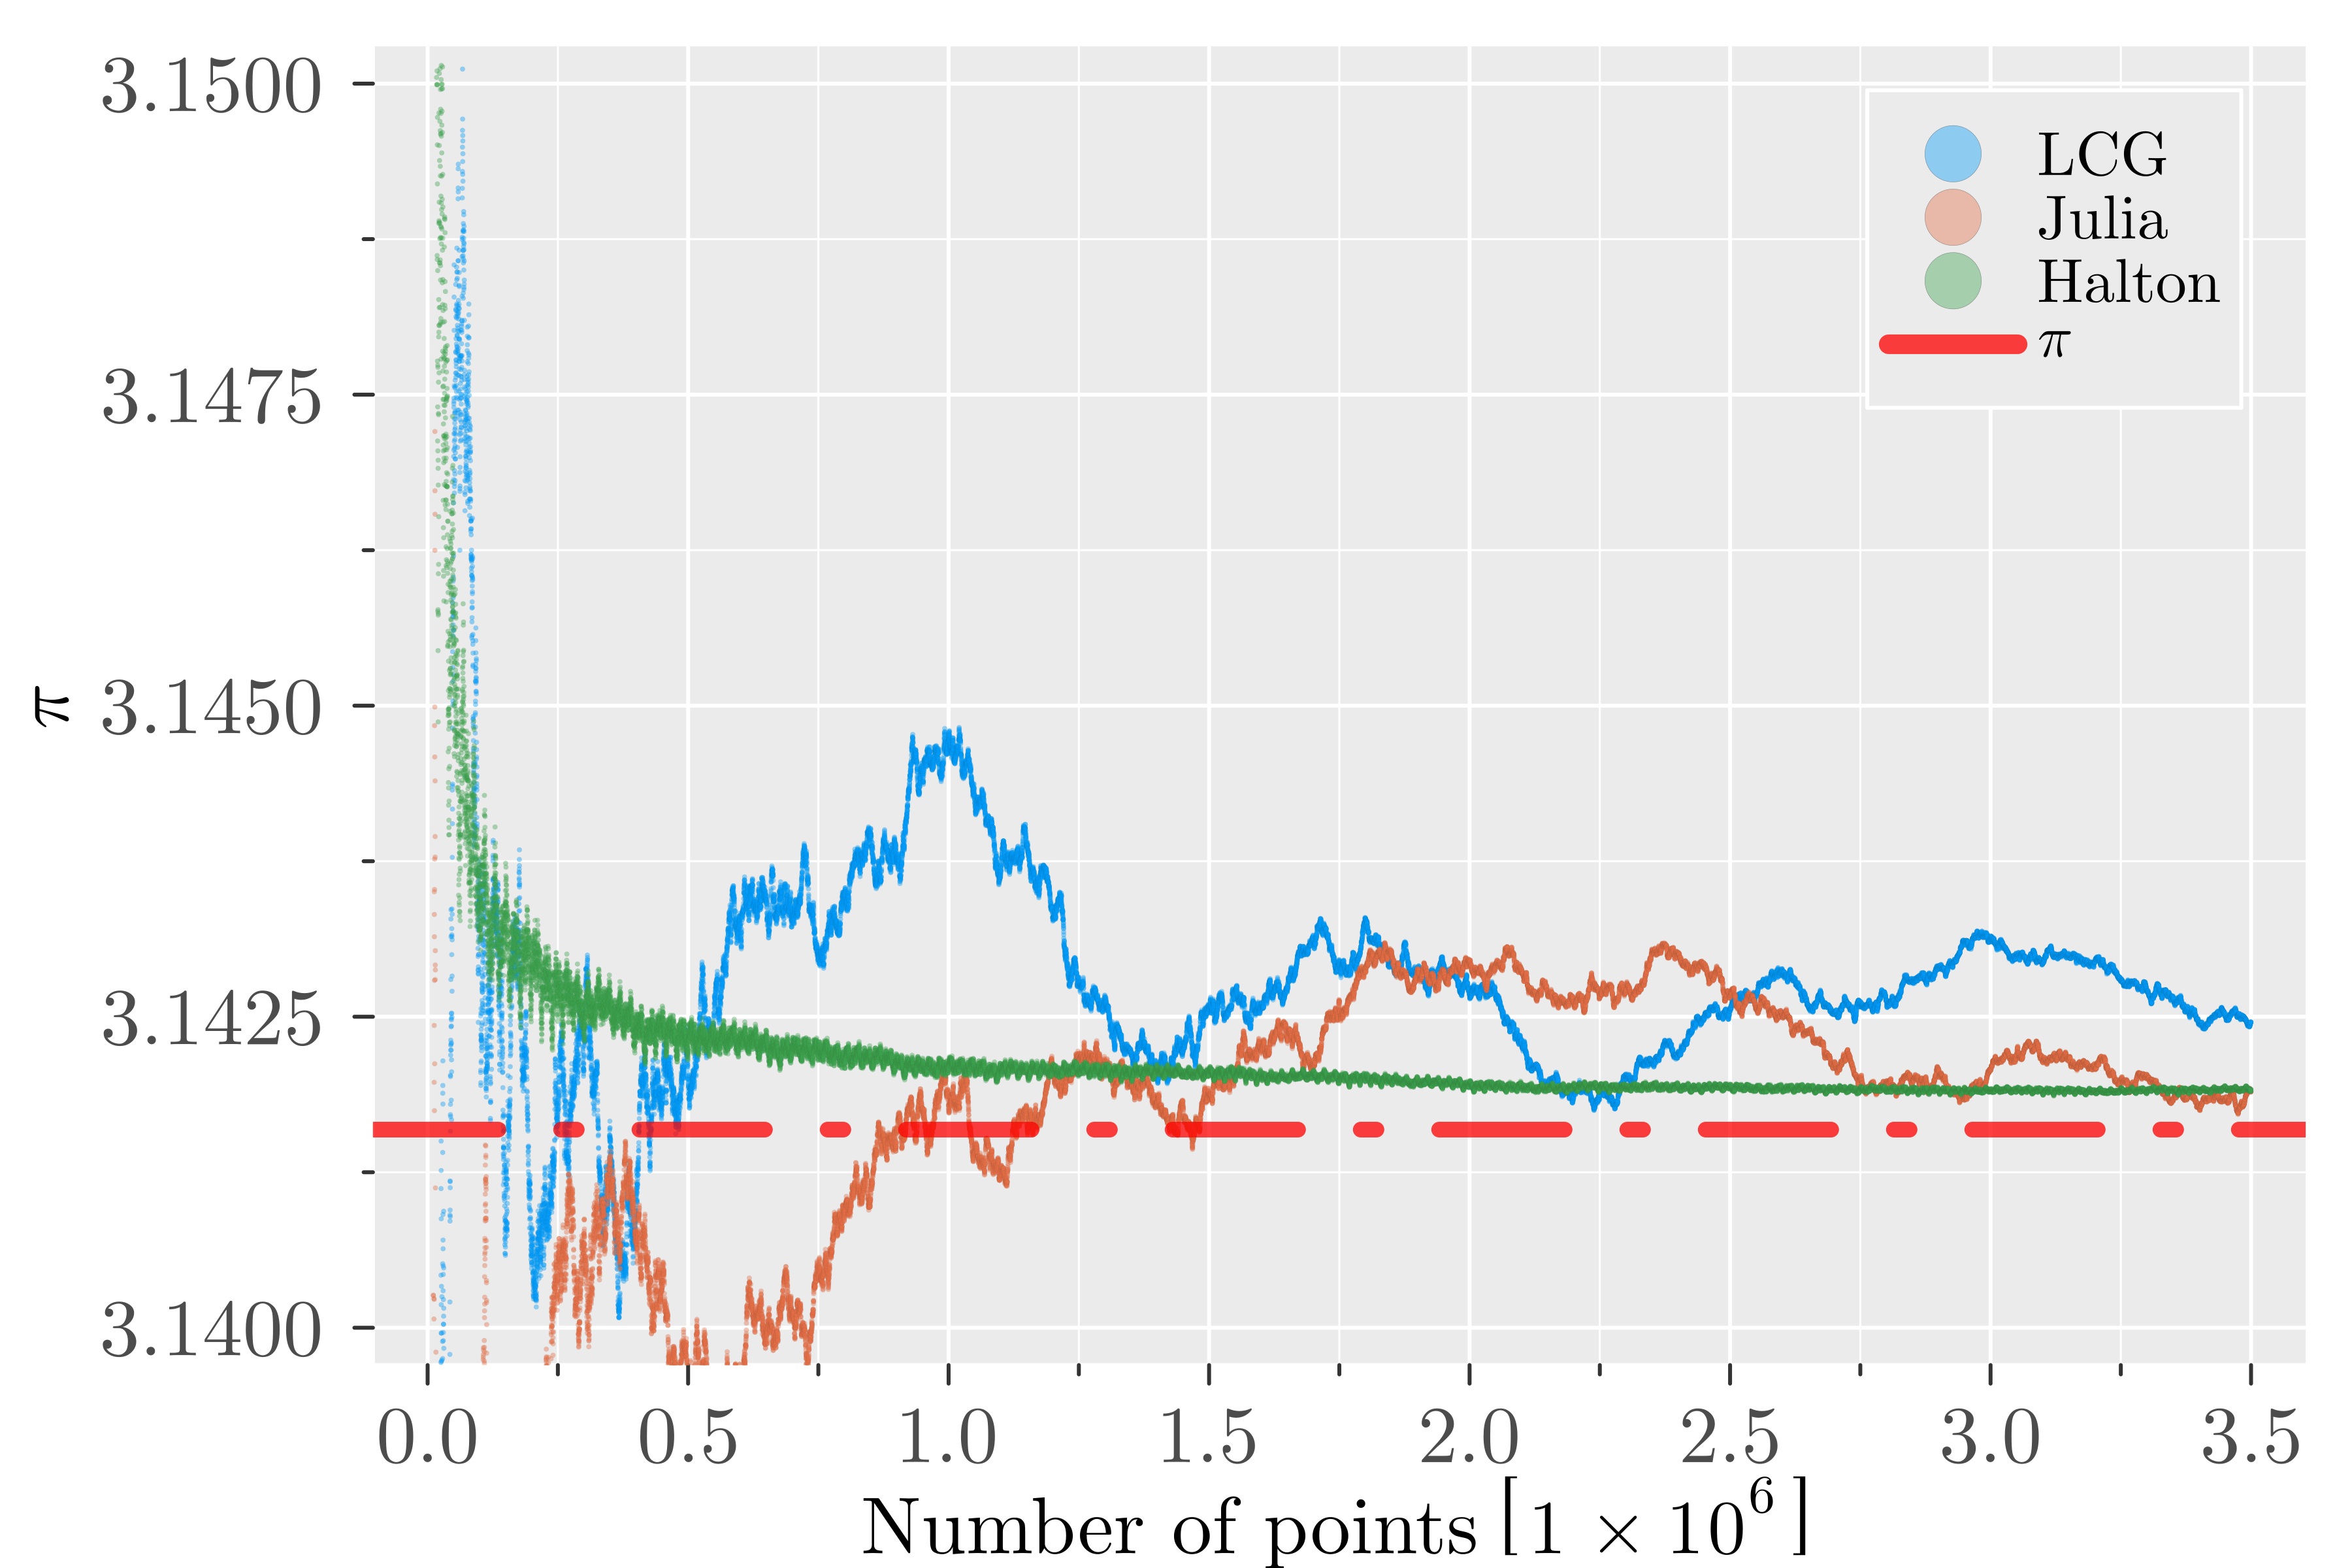
\includegraphics[scale=0.065]{../figures/pies_3dot5E6.png}
                \caption{Aproximación de $\pi$ con $3.5 \times 10^6$ puntos.}
            \end{subfigure}
            %
            \begin{subfigure}{0.45\textwidth}
                \centering
                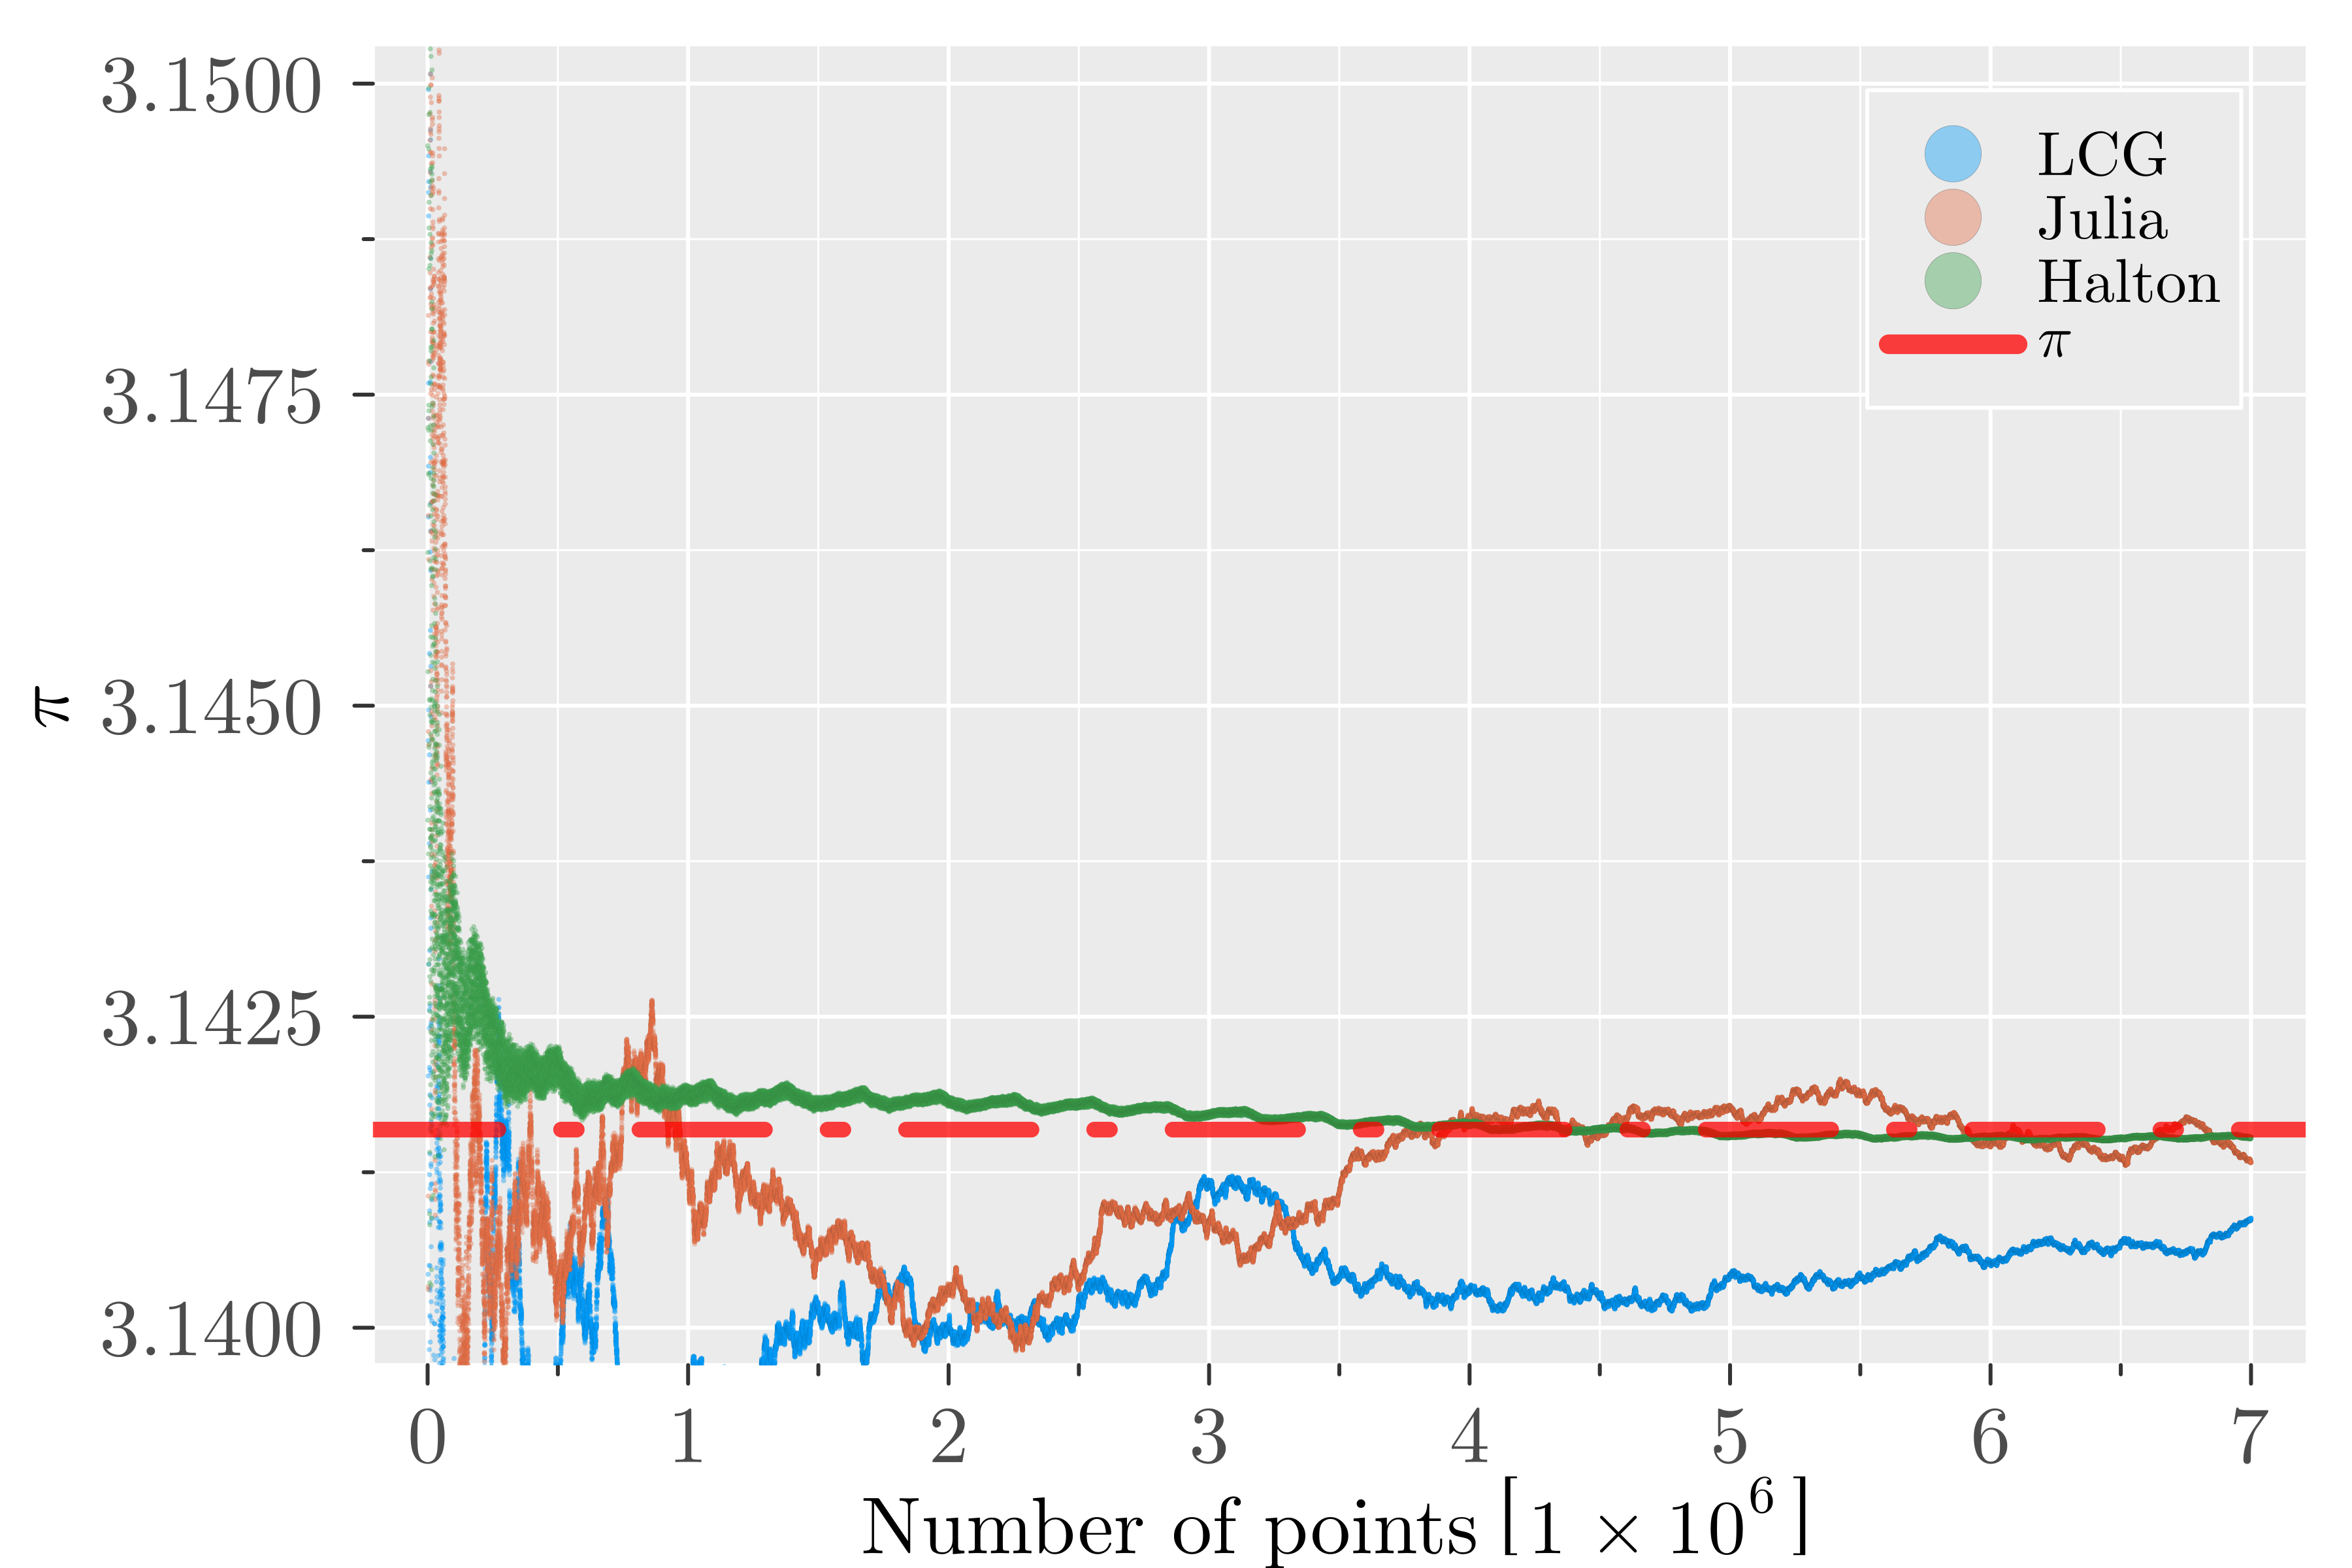
\includegraphics[scale=0.065]{../figures/pies_7E6.png}
                \caption{Aproximación de $\pi$ con $7 \times 10^6$ puntos.}
            \end{subfigure}
            \hfill
            \begin{subfigure}{0.45\textwidth}
                \centering
                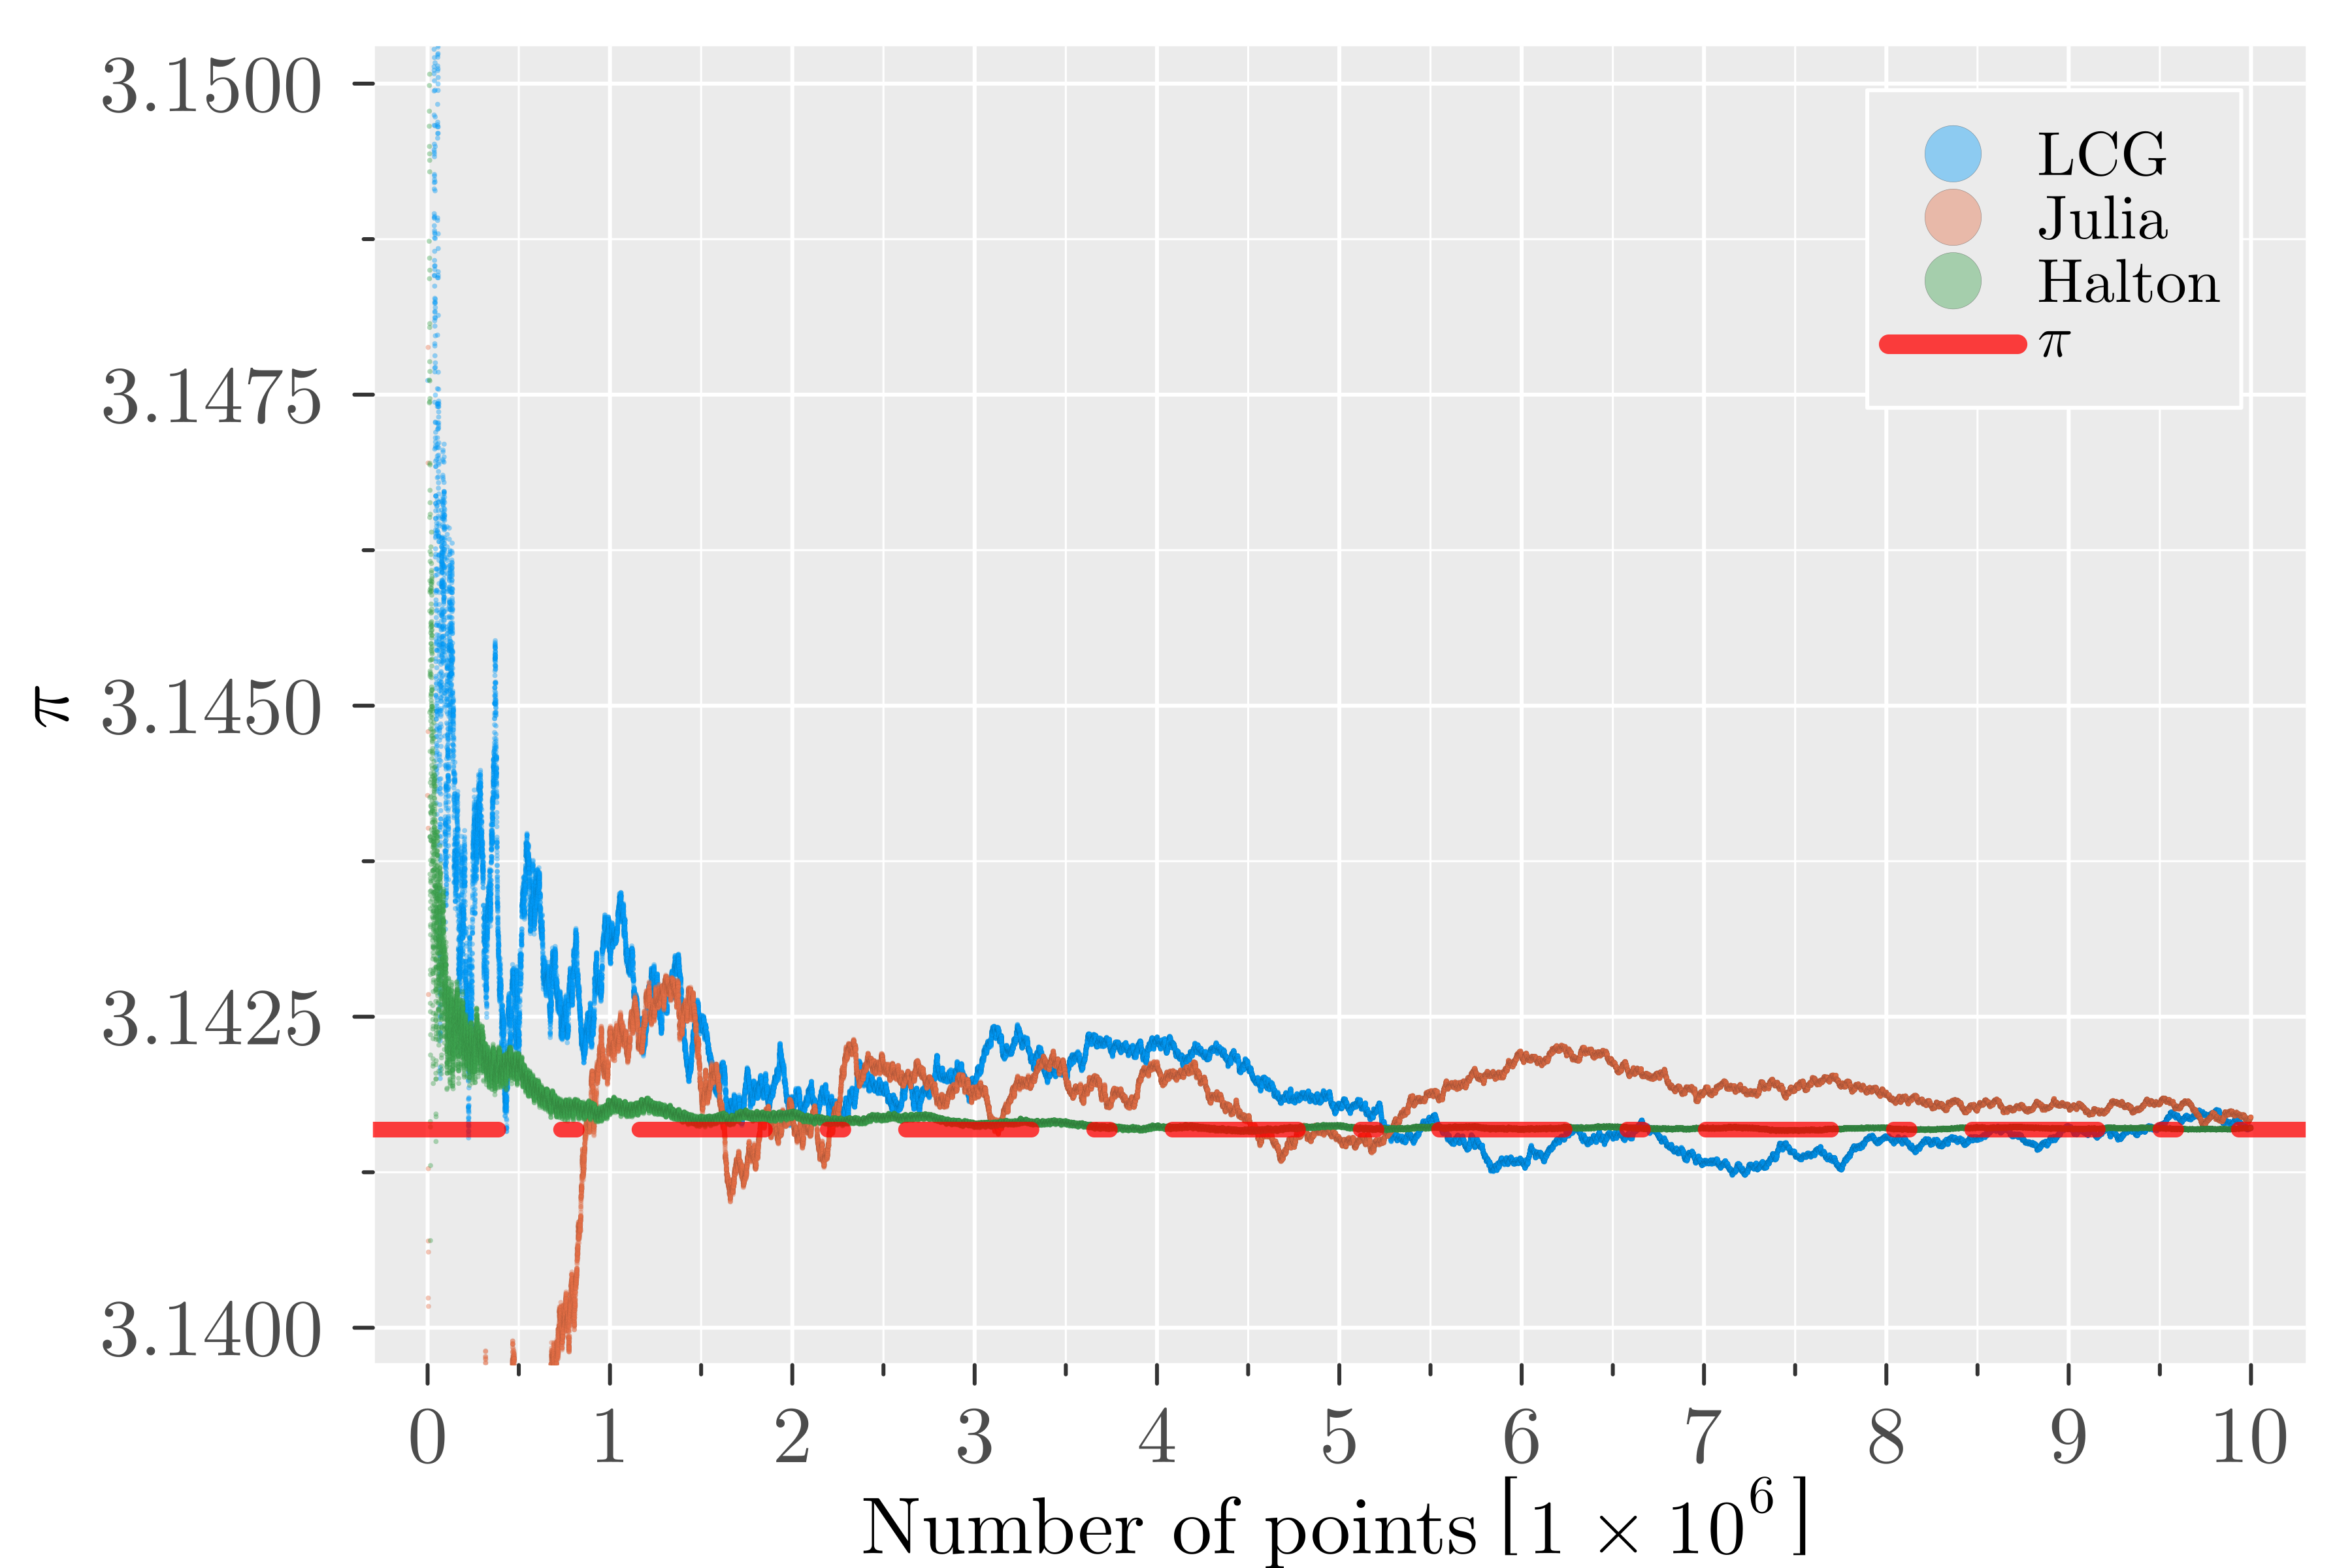
\includegraphics[scale=0.065]{../figures/pies_10E6.png}
                \caption{Aproximación de $\pi$ con $10 \times 10^6$ puntos.}
            \end{subfigure}
            %
            \caption{Gráficas de las aproximaciones de $\pi$ variando el total de puntos.}
            \label{fig:pi_approximations}
        \end{figure}

        \clearpage
        \begin{figure}
            \centering
            \begin{subfigure}{0.45\textwidth}
                \centering
                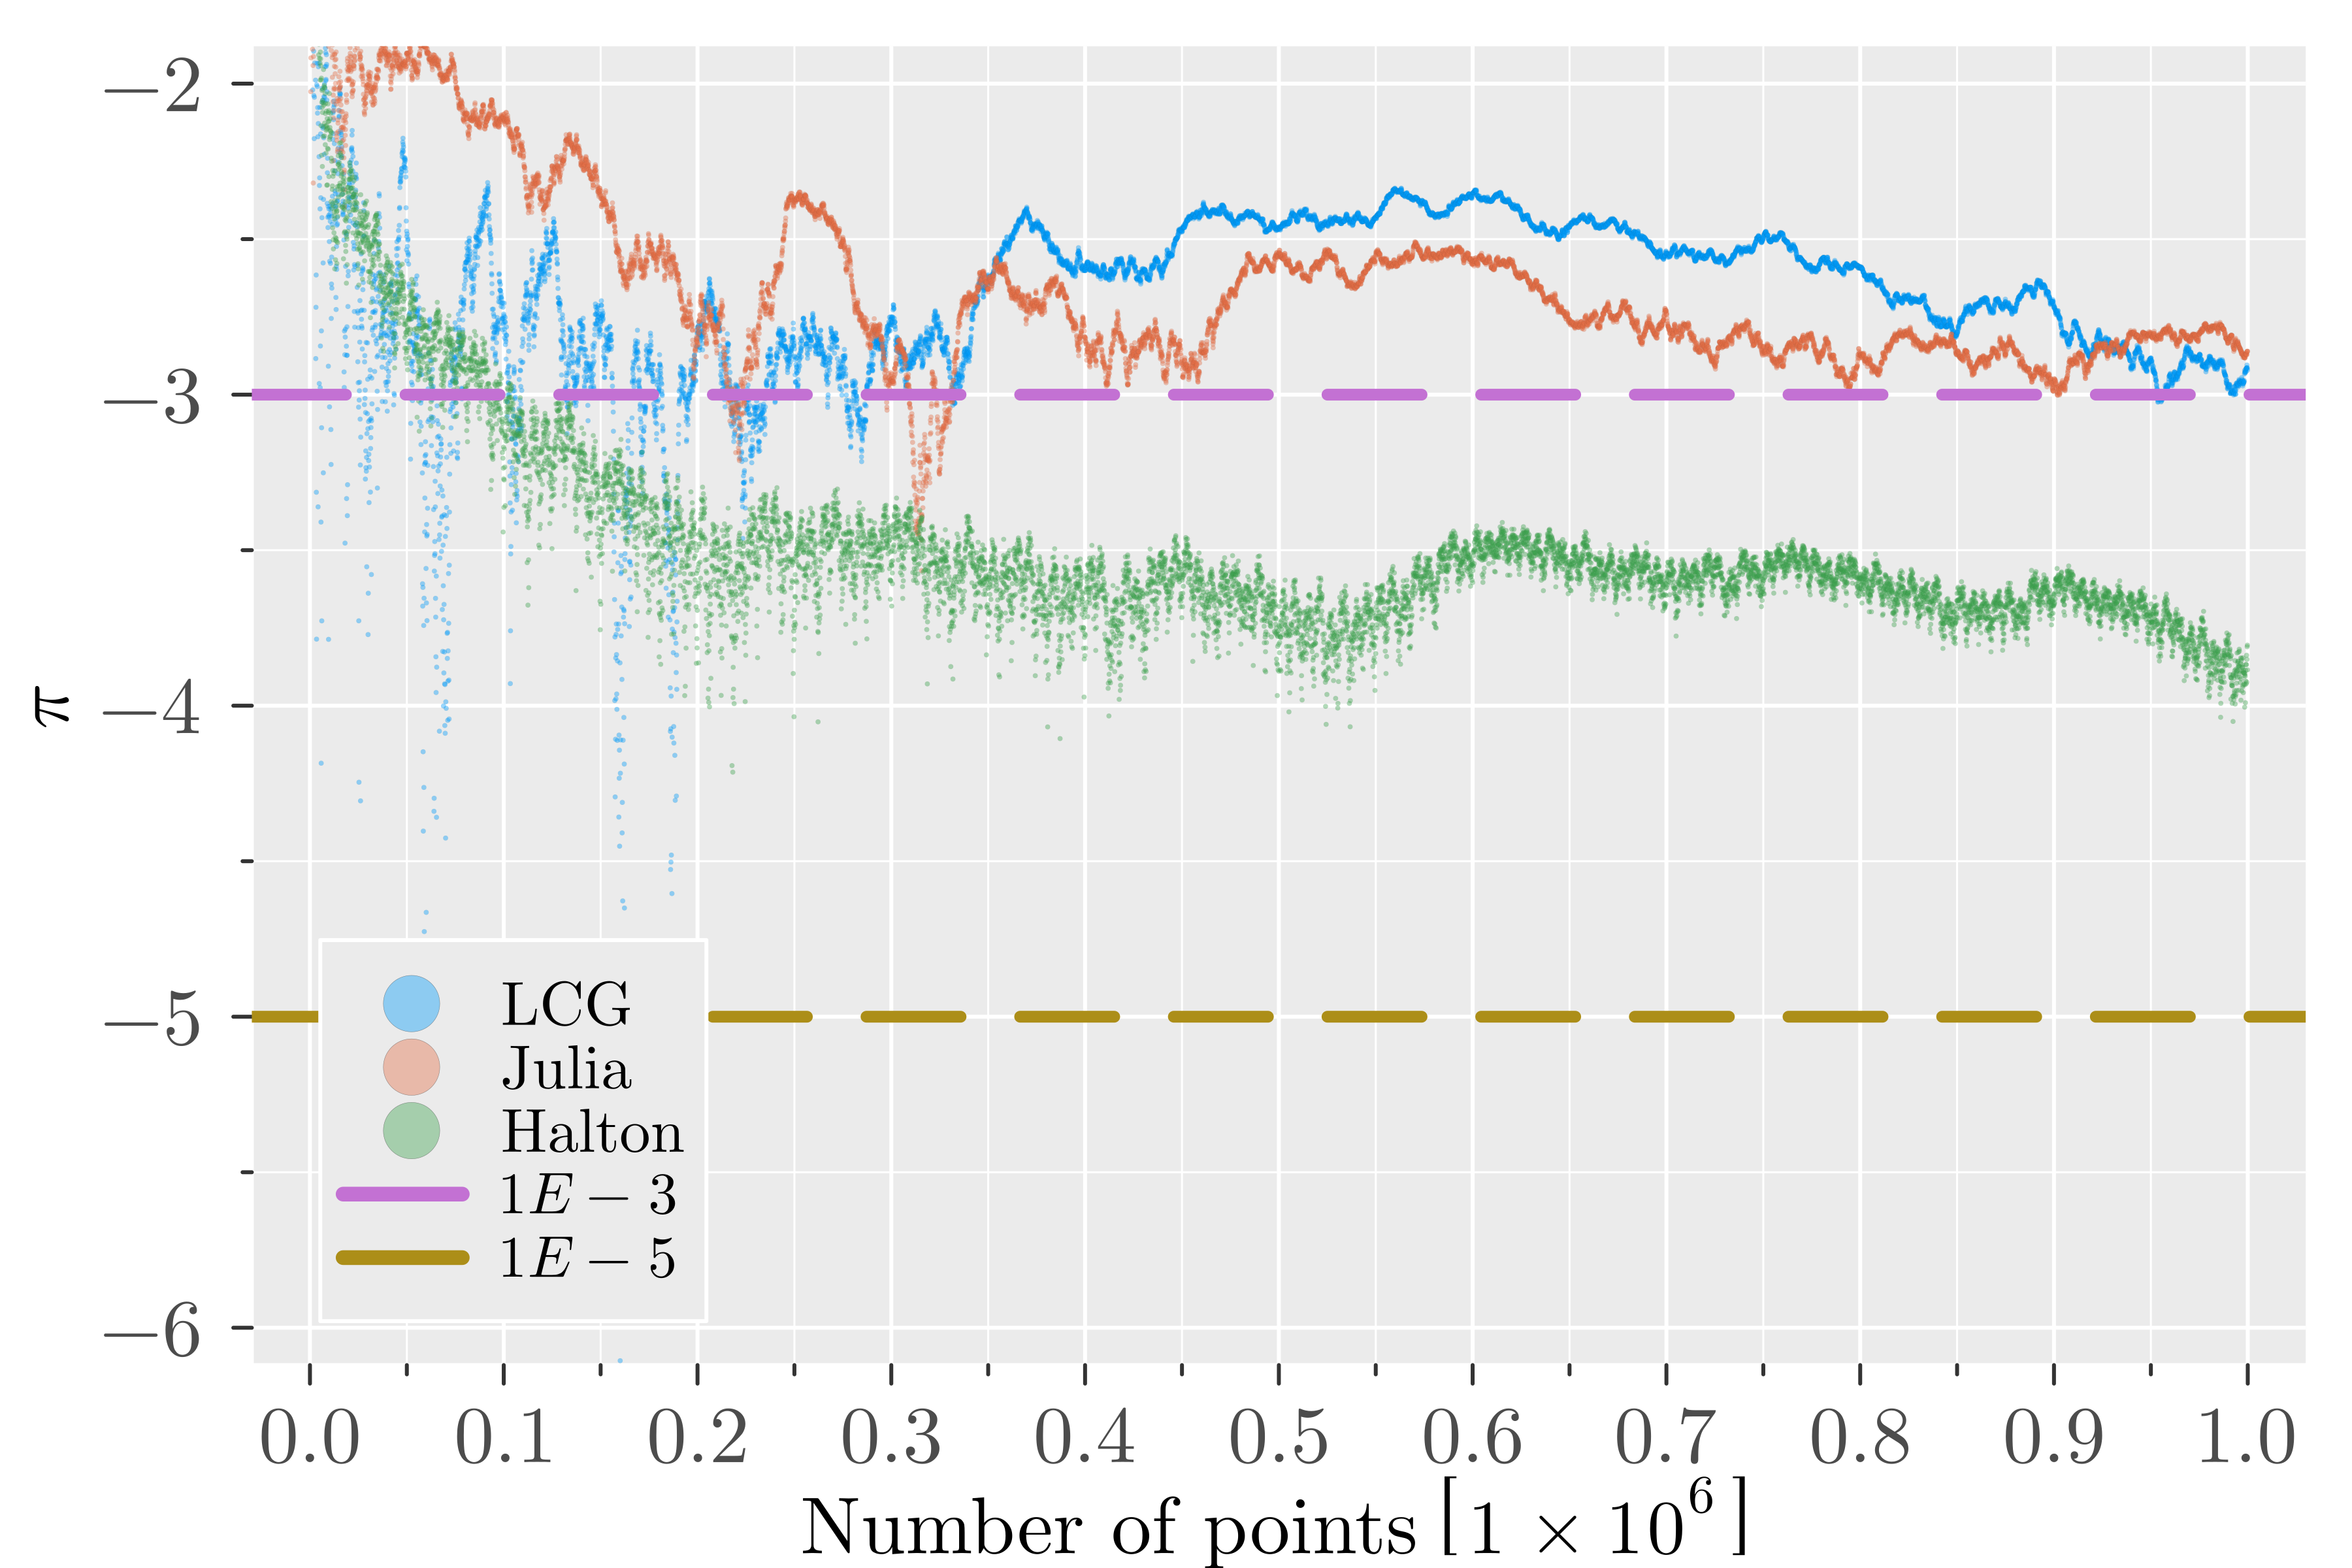
\includegraphics[scale=0.065]{../figures/error_1E6.png}
                \caption{Error de $\pi$ con $1 \times 10^6$ puntos.}
            \end{subfigure}
            \hfill
            \begin{subfigure}{0.45\textwidth}
                \centering
                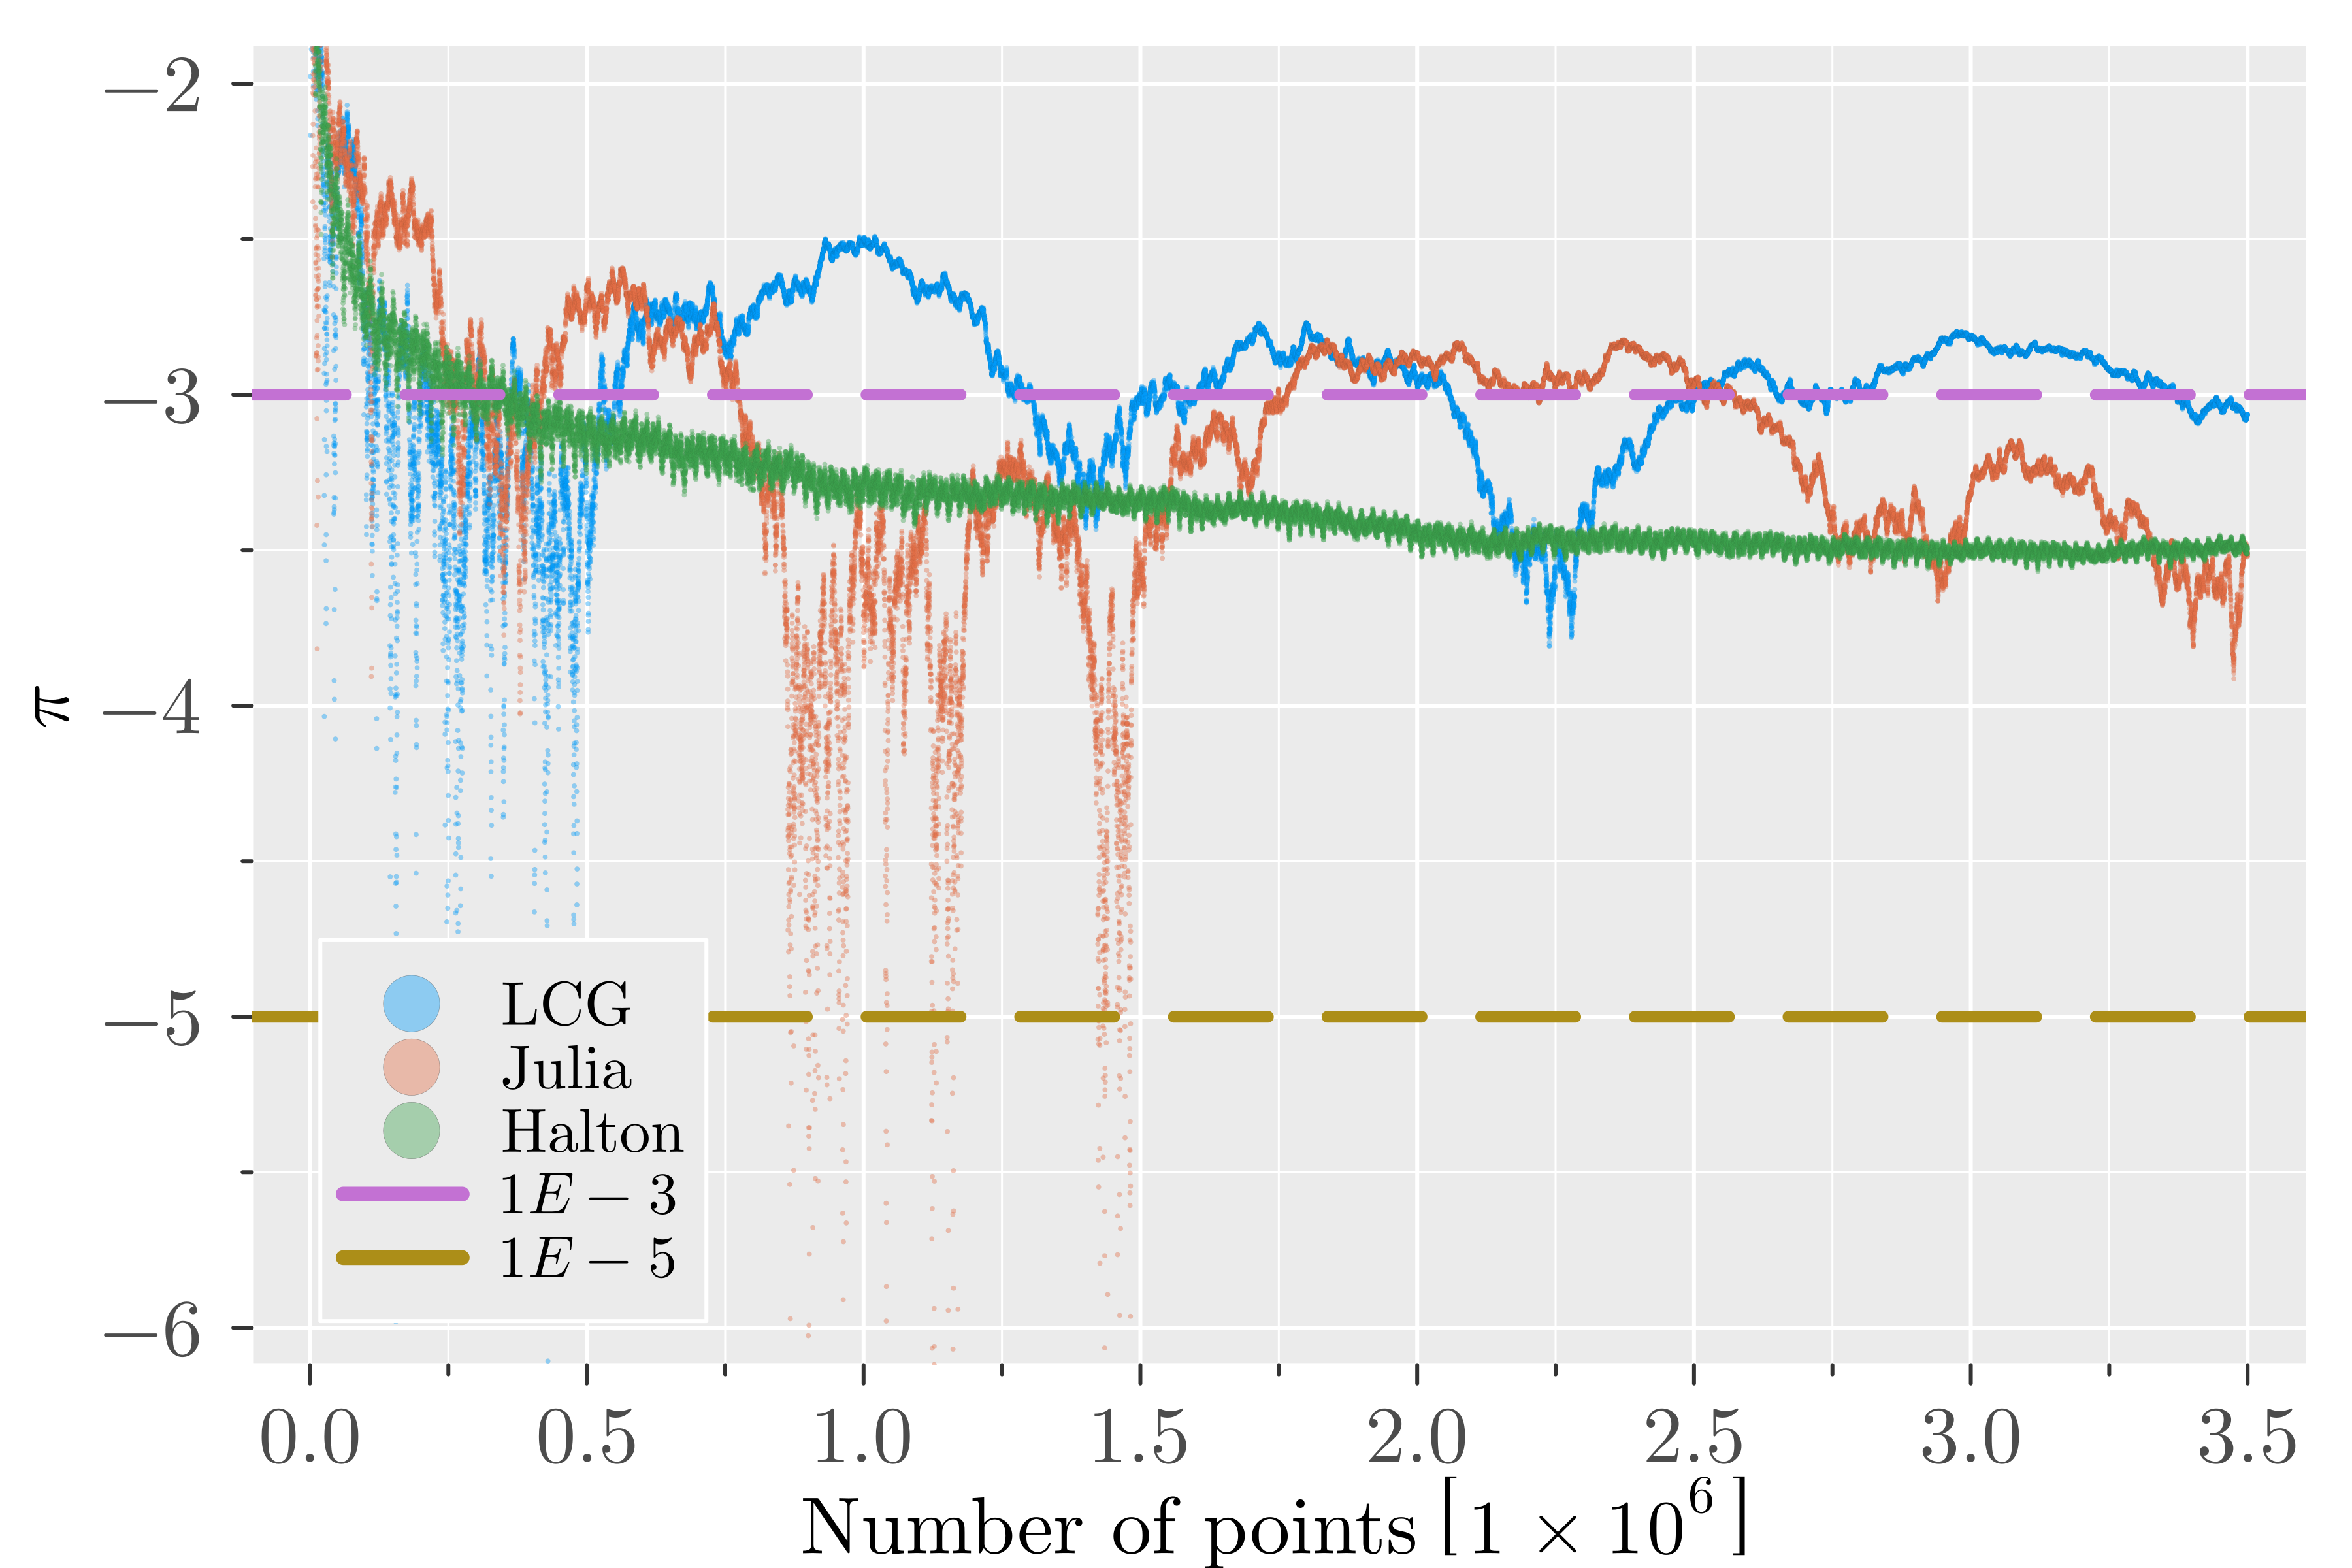
\includegraphics[scale=0.065]{../figures/error_3dot5E6.png}
                \caption{Error de $\pi$ con $3.5 \times 10^6$ puntos.}
            \end{subfigure}
            %
            \begin{subfigure}{0.45\textwidth}
                \centering
                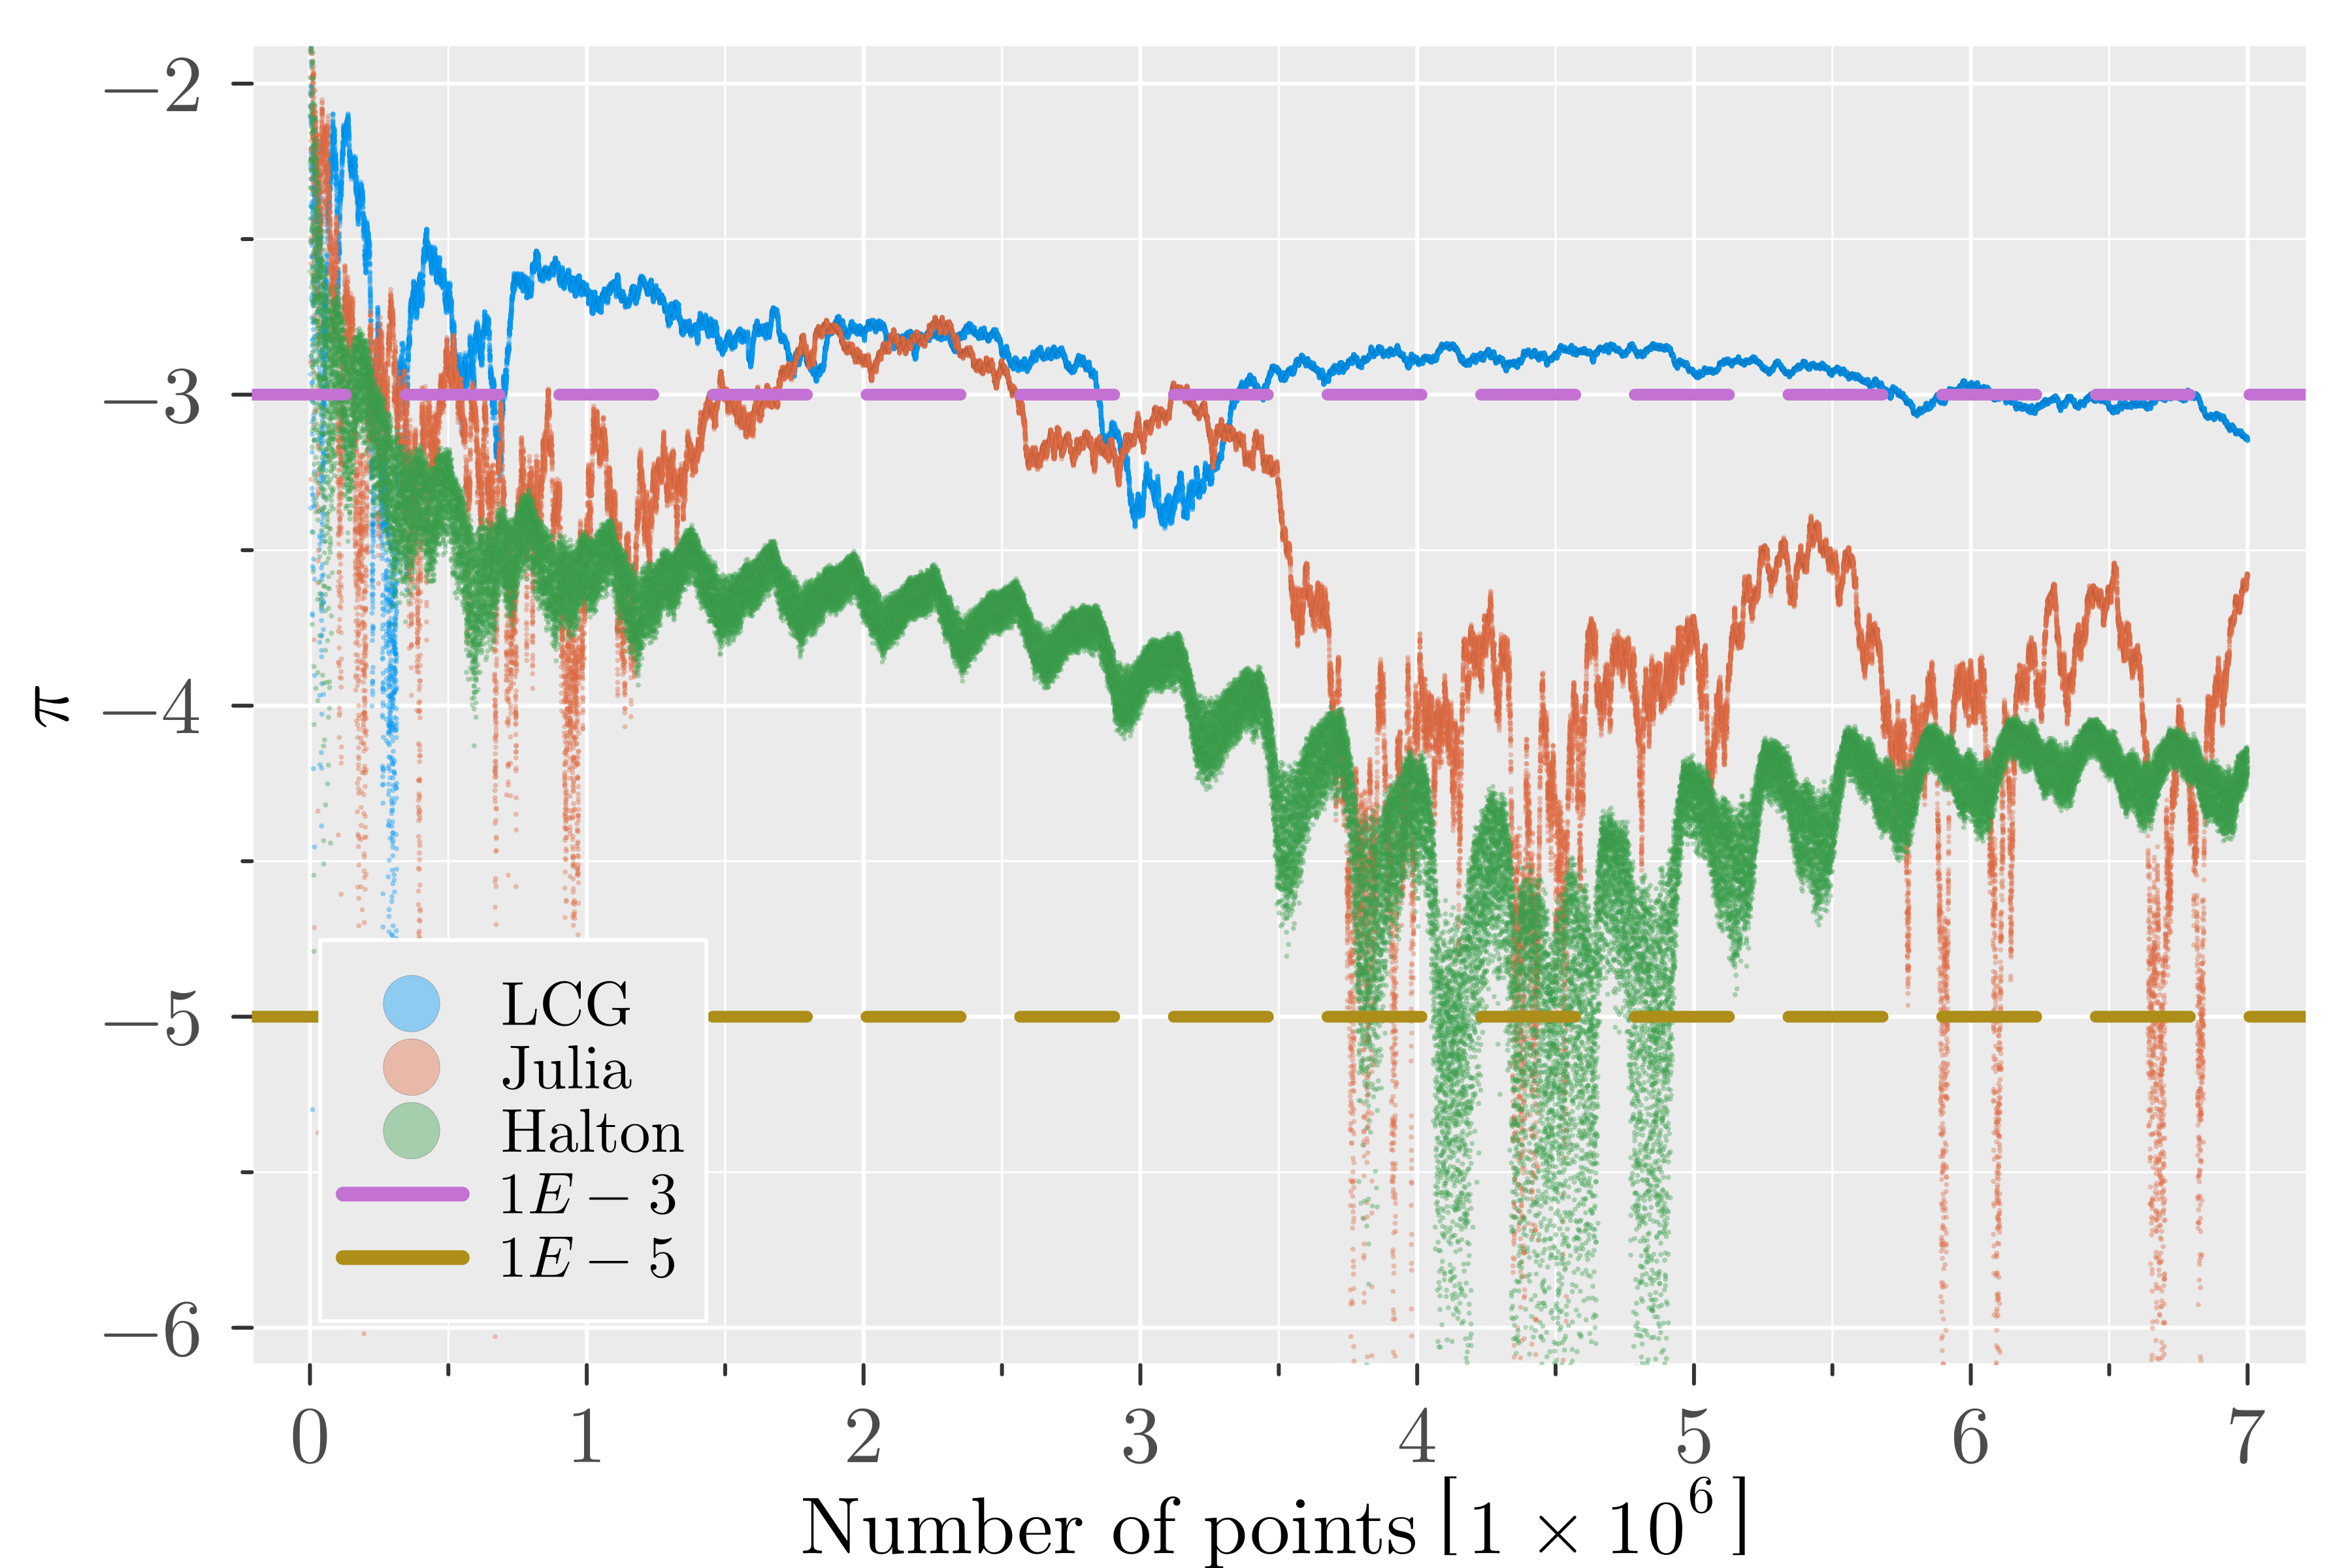
\includegraphics[scale=0.065]{../figures/error_7E6.png}
                \caption{Error de $\pi$ con $7 \times 10^6$ puntos.}
            \end{subfigure}
            \hfill
            \begin{subfigure}{0.45\textwidth}
                \centering
                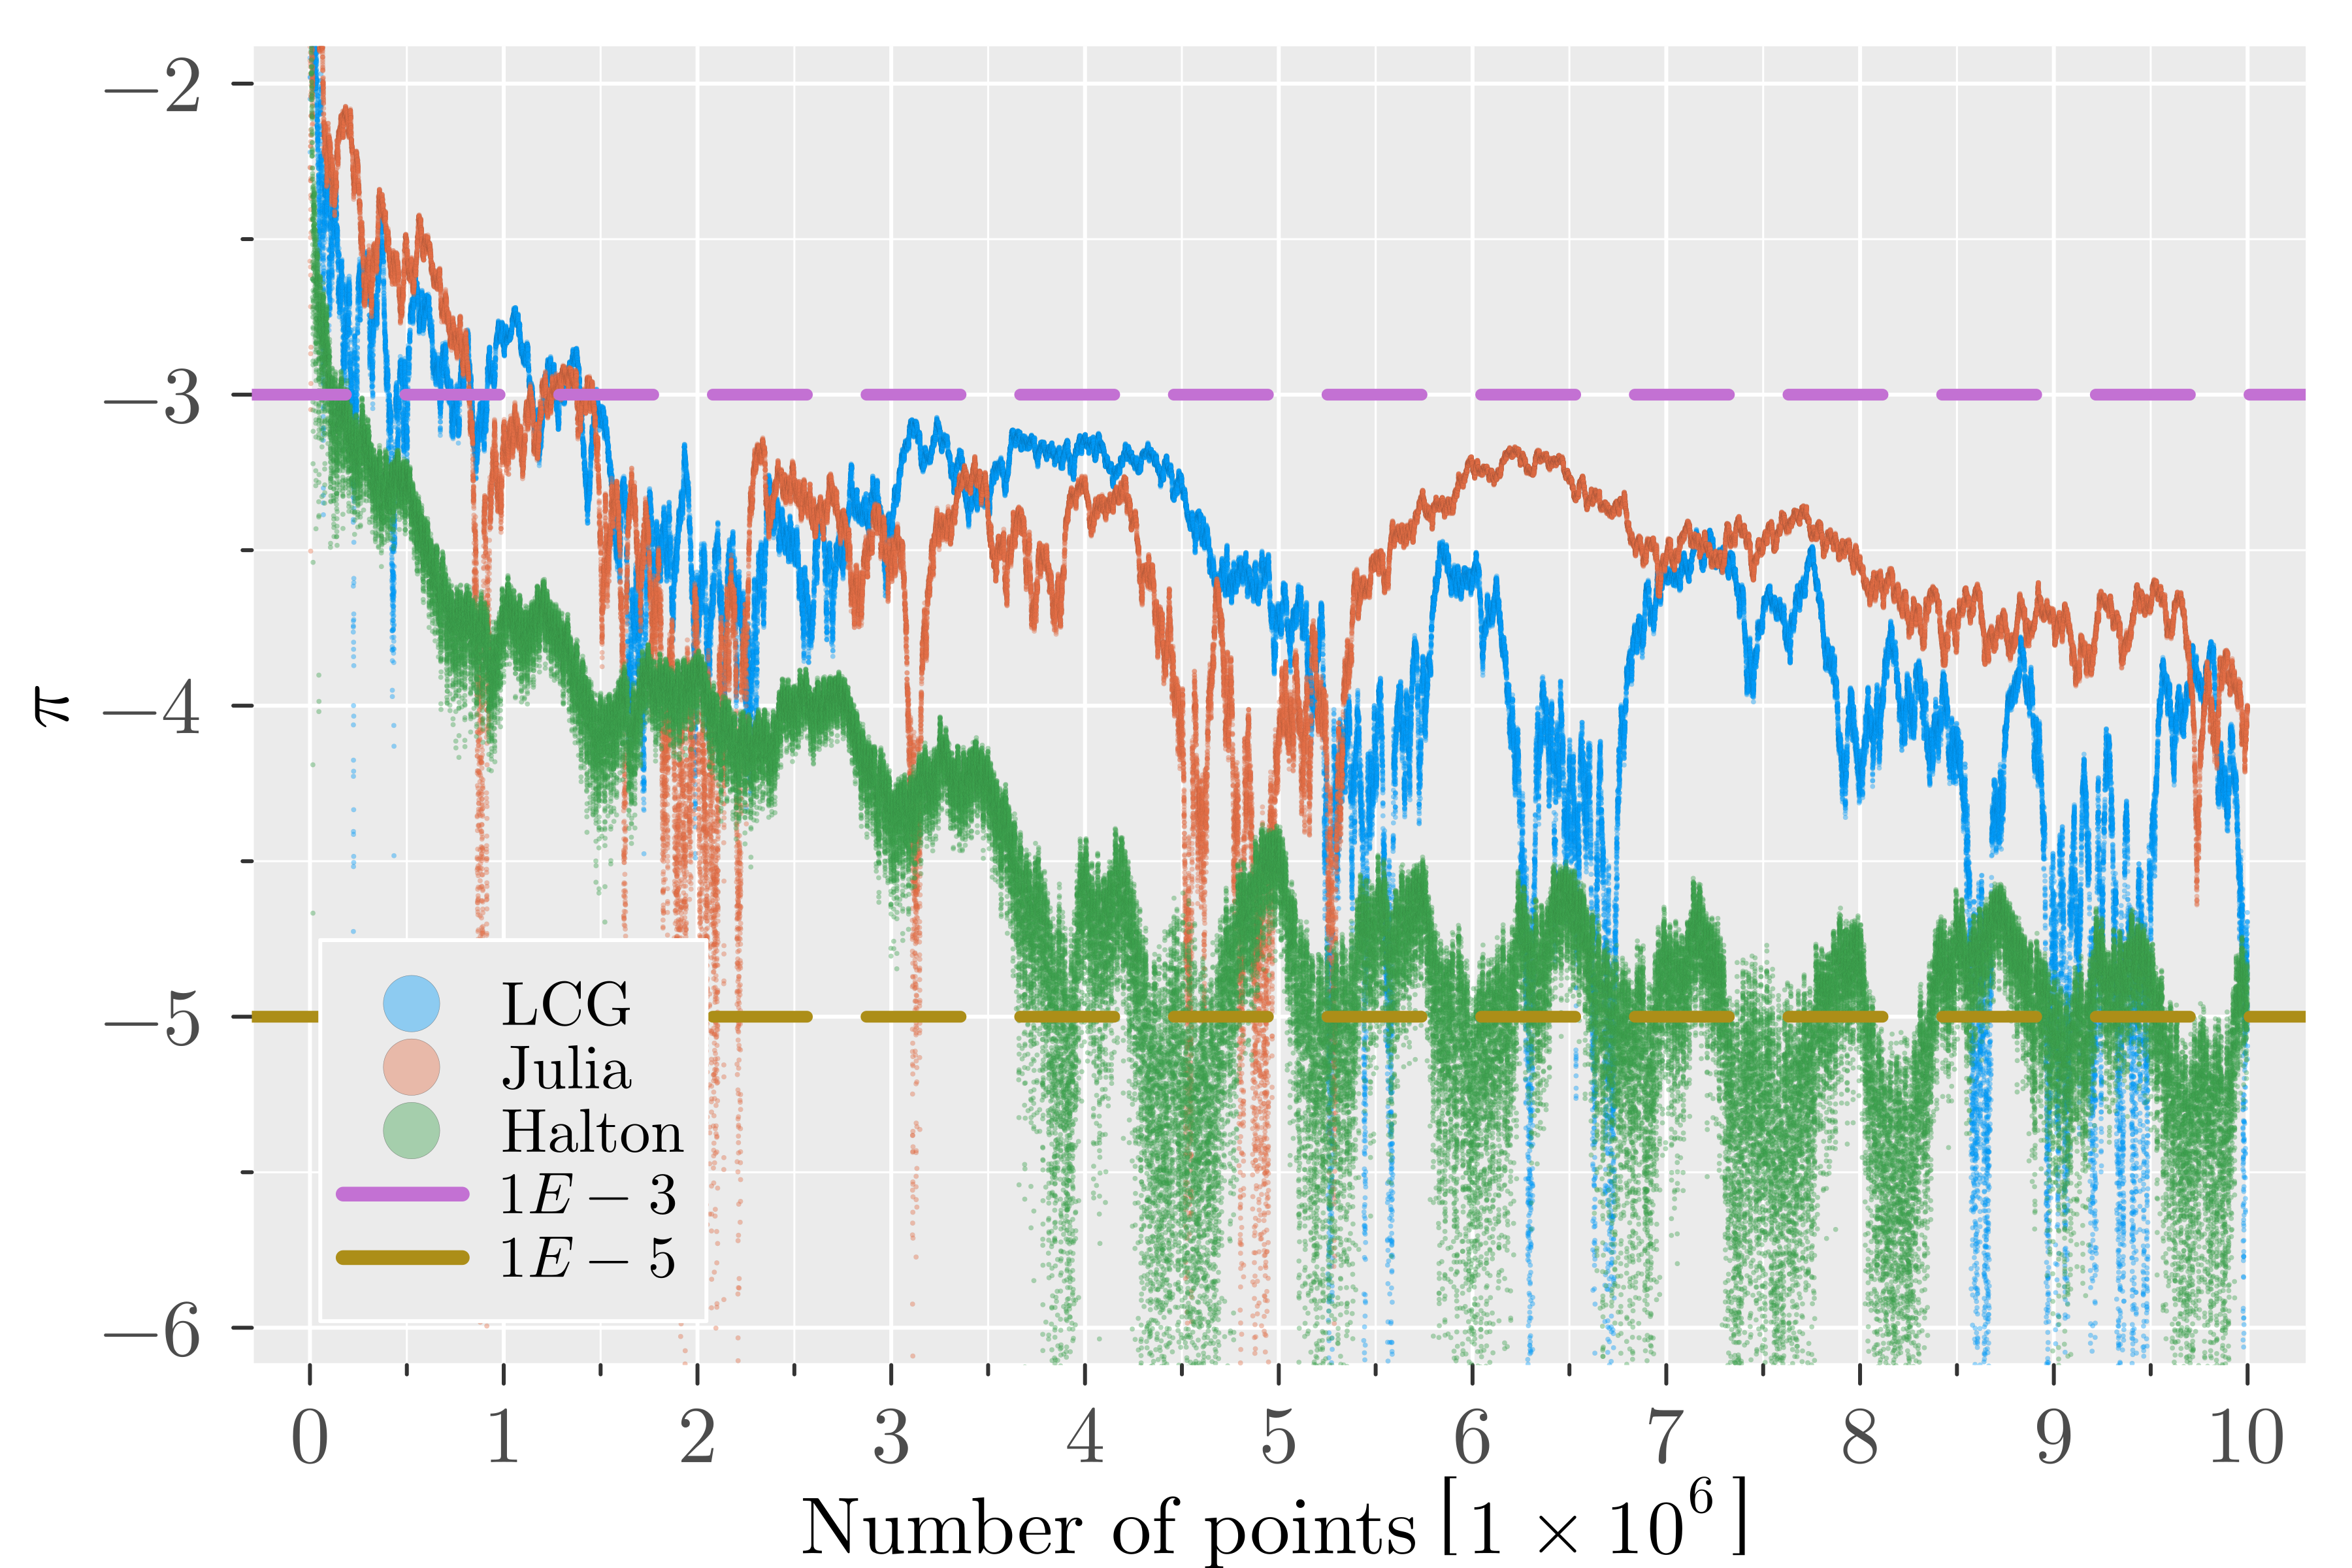
\includegraphics[scale=0.065]{../figures/error_10E6.png}
                \caption{Error de $\pi$ con $10 \times 10^6$ puntos.}
            \end{subfigure}
            %
            \caption{Gráficas correspondientes al error de las aproximaciones.}
            \label{fig:pi_errors}
        \end{figure}

    \end{solution}
\end{enumerate}

\clearpage
\section*{Apéndice}
\inputminted[
    frame=none,
    autogobble,
    obeytabs=false,
    breaklines,
    tabsize=4,
    linenos=true,
    baselinestretch=1,
    firstnumber=1,
    bgcolor=bg!70,]{julia}{\codepath}

\nocite{*}    % to call all references even if they are not cited in the text
\bibliography{references.bib}

\end{document}

% \begin{minted}[
%     frame=none,
%     autogobble,
%     obeytabs=false,
%     breaklines,
%     tabsize=4,
%     linenos=true,
%     baselinestretch=1,
%     firstnumber=1,
%     bgcolor=bg!70,
%     ]{julia}
%     # Pseudocodigo
%     # Vecino arriba
%     if id > nc
%         agrega (id - nc) como vecino
%     end if
%     # Vecino abajo
%     if id <= nc * (nr - 1)
%         agrega (id + nc) como vecino
%     end if
% \end{minted}



% ----------------------------------------------------------------------------
% 1E6
% ----------------------------------------------------------------------------
% julia> (err_lcg[end], err_jul[end], err_halt[end])
% (0.0011913464102067615373566167204971158028306006248941790250554076921835937137966, 0.001376653589793238462643383279502884197169399375105820974944592307816406286208964, 0.0001393464102067615373566167204971158028306006248941790250554076921835937138070732)

% julia> (data_lcg.pies[end], data_jul.pies[end], data_halt.pies[end])
% (3.142783999999999999999999999999999999999999999999999999999999999999999999999995, 3.140215999999999999999999999999999999999999999999999999999999999999999999999989, 3.141732000000000000000000000000000000000000000000000000000000000000000000000005)


% ----------------------------------------------------------------------------
% 3.5E6
% ----------------------------------------------------------------------------
% julia> (data_lcg.pies[end], data_jul.pies[end], data_halt.pies[end])
% (3.14245485714285714285714285714285714285714285714285714285714285714285714285715, 3.141893714285714285714285714285714285714285714285714285714285714285714285714276, 3.141923428571428571428571428571428571428571428571428571428571428571428571428585)

% julia> (err_lcg[end], err_jul[end], err_halt[end])
% (0.0008622035530639043944994738633542586599734577677513218821982648350407365709523039, 0.0003010606959210472516423310062114015171163149106084647393411219778978794280774798, 0.0003307749816353329659280452919256872314020291963227504536268362636121651423865035)


% ----------------------------------------------------------------------------
% 7E6
% ----------------------------------------------------------------------------
% julia> (err_lcg[end], err_jul[end], err_halt[end])
% (0.0007195107326503813197862404223600270543122565179629638320874494506735491433465233, 0.0002560821612218098912148118509314556257408279465343924035160208792449777147849059, 6.751073265038131978624042236002705431225651796296383208744945067354914335721727e-05)

% julia> (data_lcg.pies[end], data_jul.pies[end], data_halt.pies[end])
% (3.140873142857142857142857142857142857142857142857142857142857142857142857142852, 3.141336571428571428571428571428571428571428571428571428571428571428571428571413, 3.141525142857142857142857142857142857142857142857142857142857142857142857142841)

% ----------------------------------------------------------------------------
% 10E6
% ----------------------------------------------------------------------------
% julia> (data_lcg.pies[end], data_jul.pies[end], data_halt.pies[end])
% (3.141603599999999999999999999999999999999999999999999999999999999999999999999986, 3.141693599999999999999999999999999999999999999999999999999999999999999999999989, 3.141603999999999999999999999999999999999999999999999999999999999999999999999987)

% julia> (err_lcg[end], err_jul[end], err_halt[end])
% (1.09464102067615373566167204971158028306006248941790250554076921835937137877954e-05, 0.0001009464102067615373566167204971158028306006248941790250554076921835937137912996, 1.134641020676153735661672049711580283060062489417902505540769218359371378903923e-05)